\documentclass{standalone}
\usepackage{tikz}
\begin{document}
    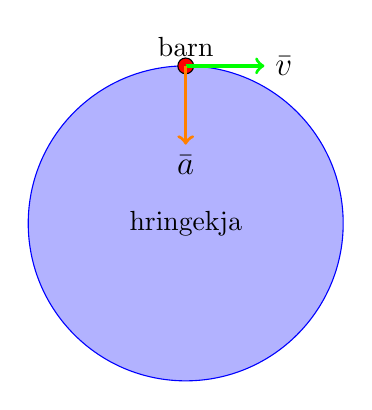
\begin{tikzpicture}
        \draw [draw=blue, fill=blue, fill opacity=0.3] (4,4) circle [radius=2] node [black, opacity=1] {hringekja};
        \draw [fill=red] (4,6) circle [radius=0.1] node [above] {barn};
        \draw [very thick, green, ->] (4,6) -- (5,6) node [right, black] {\large $\bar{v}$};
        \draw [very thick, orange, ->] (4,6) -- (4,5) node [below, black] {\large $\bar{a}$};
    \end{tikzpicture}
\end{document}
